\documentclass[10pt,a4paper,twocolumn]{article}
\usepackage[utf8]{inputenc}
\usepackage[english]{babel}
\usepackage{amsmath}
\usepackage{amsfonts}
\usepackage{amssymb}
\usepackage{graphicx}
\usepackage{url}
\usepackage[colorlinks=true, allcolors=blue]{hyperref}
\usepackage{booktabs}
\usepackage{float}
\usepackage{natbib}
\usepackage[left=2cm,right=2cm,top=2cm,bottom=2cm]{geometry}

\title{Reducing Demand for Critical Materials through Electric Vehicle Battery Recycling: An Agent-Based Modeling Study}

\author{
        Your Name\\
        Your Institution\\
        \texttt{your.email@institution.com}
}

\date{\today}

\begin{document}

\maketitle

\begin{abstract}
Electric vehicle (EV) adoption is growing rapidly worldwide, increasing the demand for critical materials like lithium and cobalt used in their batteries. This study develops an agent-based model to investigate how recycling can reduce the demand for these materials. The model simulates interactions between EV owners, battery manufacturers, and recycling companies over a period from 2024 to 2050. Various scenarios are explored, including baseline recycling rates, no recycling, and high-efficiency recycling. Results indicate that with baseline recycling parameters, lithium demand can be reduced by approximately 42\%, and cobalt demand by approximately 44\% by 2050 compared to a no-recycling scenario. The high-efficiency scenario demonstrates even greater potential for demand reduction. This paper contributes to understanding the resource implications of large-scale EV adoption and the importance of developing efficient recycling infrastructure to support sustainable transportation systems.
\end{abstract}

\section{Introduction}
\label{sec:introduction}

The transition to electric mobility represents one of the most significant shifts in the transportation sector. As the global fleet of electric vehicles (EVs) grows, so does the demand for the materials used in their batteries, particularly lithium and cobalt \citep{olivetti2017}. These materials face supply constraints due to geographic concentration, geopolitical factors, and environmental concerns associated with mining practices \citep{dominish2019}.

Recycling has been proposed as a key strategy for reducing the primary demand for these materials \citep{harper2019}, creating a more circular economy for battery materials. However, the extent to which recycling can offset new material demand depends on multiple interconnected factors: the growth rate of the EV market, the efficiency of recycling processes, consumer decisions to recycle end-of-life batteries, and the lifespan of batteries.

This paper addresses the research question: \textit{"How much can the demand for lithium and cobalt decrease if we recycle electric vehicle batteries?"}. To answer this question, we develop an agent-based model (ABM) that simulates the dynamic interactions between EV owners, battery manufacturers, and recycling companies. Agent-based modeling is particularly suitable for this research as it can capture emergent behavior from complex interactions between heterogeneous agents operating under different decision rules \citep{bonabeau2002}.

The results provide insights into the potential material savings from recycling and highlight the importance of policies that encourage both improved recycling technologies and higher rates of consumer participation in recycling programs.

\section{Background}
\label{sec:background}

\subsection{Electric Vehicle Battery Materials}

Lithium-ion batteries are the dominant technology used in electric vehicles, with lithium and cobalt being critical components. Lithium is primarily used in the battery cathode and electrolyte, while cobalt is used in the cathode to improve stability and energy density \citep{xu2017}. 

A typical EV battery contains approximately 2.5 kg of lithium and 6 kg of cobalt, though this varies by battery chemistry and vehicle type \citep{ellingsen2016}. The concentration of these materials makes EV batteries valuable for recycling, especially given that cobalt resources are geographically concentrated, with over 70\% of global production coming from the Democratic Republic of Congo \citep{usgs2020}.

\subsection{Growth of the EV Market}

The global EV market is projected to grow significantly in the coming decades. Various forecasts estimate annual growth rates between 8-12\% for 2024-2030, accelerating to 12-18\% for 2030-2035, and then moderating to 5-10\% for 2035-2050 \citep{elaadoutlook}. This growth is driven by policy measures (including internal combustion engine bans in several countries), declining battery costs, and increasing consumer acceptance.

\subsection{Battery Recycling Technologies}

Current recycling processes for lithium-ion batteries include pyrometallurgical (high-temperature) and hydrometallurgical (chemical leaching) methods \citep{zheng2018}. Current commercial recycling processes can recover approximately 60-70\% of lithium and cobalt from batteries, with ongoing research aiming to improve these rates \citep{dunn2021}. Annual improvements in recycling efficiency of 2-3\% are considered achievable based on current technological trajectories \citep{rmi2022}.

\subsection{Consumer Recycling Behavior}

Consumer decision-making regarding battery recycling is influenced by multiple factors, including awareness, convenience, financial incentives, and social norms \citep{sun2020}. Network effects play an important role, as awareness and acceptance of recycling practices spread through social networks \citep{axsen2013}.

\section{Methodology}
\label{sec:methodology}

\subsection{Agent-Based Model Design}

We developed an agent-based model using the Mesa framework in Python to simulate the EV battery lifecycle and recycling system. The model consists of three types of agents: EV owners, battery manufacturers, and recycling companies. These agents interact within an environment defined by market growth parameters, recycling efficiencies, and material flows.

\subsubsection{EV Owners}

EV owners are agents who possess electric vehicles with batteries that age over time. Each battery has a lifespan of 8 years before reaching 80\% capacity, at which point the owner decides whether to recycle or discard the battery. This decision is probabilistic and influenced by both individual preferences and network effects. Each owner's likelihood of recycling increases gradually over time as social awareness about recycling grows.

\subsubsection{Battery Manufacturers}

Battery manufacturers produce new batteries to meet demand from both new EV sales and replacement batteries. They preferentially use recycled materials when available before sourcing new (virgin) materials. Each battery requires 2.5 kg of lithium and 6 kg of cobalt.

\subsubsection{Recycling Companies}

Recycling companies process end-of-life batteries to recover lithium and cobalt. The efficiency of this process starts at 60\% in 2024 and increases by 2.5\% annually, capped at a maximum efficiency of 98\%. Recovered materials are returned to the market for use in new batteries.

\subsection{Model Parameters}

The model uses the following key parameters:

\begin{table}[h]
\centering
\caption{Key Model Parameters}
\begin{tabular}{ll}
\toprule
Parameter & Value \\
\midrule
Initial EV owners & 1,000 \\
Battery lifespan & 8 years (to 80\% capacity) \\
Lithium content per battery & 2.5 kg \\
Cobalt content per battery & 6.0 kg \\
Initial recycling efficiency & 60\% \\
Annual efficiency improvement & 2.5\% \\
Base recycling probability & 50\% \\
EV market growth (2024-2030) & 10\% per year \\
EV market growth (2031-2035) & 15\% per year \\
EV market growth (2036-2050) & 7.5\% per year \\
\bottomrule
\end{tabular}
\label{tab:parameters}
\end{table}

\subsection{Scenarios}

We explored three scenarios to assess the impact of recycling on material demand:

\begin{enumerate}
    \item \textbf{Baseline}: Default recycling parameters (50\% recycling probability, starting at 60\% efficiency with 2.5\% annual improvement).
    \item \textbf{No Recycling}: Zero recycling probability and efficiency, representing a counterfactual where batteries are not recycled.
    \item \textbf{High Efficiency}: Higher recycling probability (80\%) and efficiency (starting at 80\% with 4\% annual improvement), representing an optimistic scenario with technological advances and strong policy support.
\end{enumerate}

\subsection{Data Collection and Analysis}

The model tracks the following metrics over the simulation period:

\begin{itemize}
    \item Number of EVs in use
    \item Recycling efficiency over time
    \item New lithium and cobalt required (kg)
    \item Recycled lithium and cobalt available (kg)
\end{itemize}

The simulation runs from 2024 to 2050, with each step representing one year. For each scenario, the model was run once due to the deterministic nature of the macro-level outcomes, though individual agent decisions contain stochastic elements.

\section{Results}
\label{sec:results}

\subsection{Material Demand Reduction}

The model results show a significant potential for recycling to reduce demand for virgin lithium and cobalt. Figure \ref{fig:lithium_demand} shows the new lithium demand over time across all three scenarios, while Figure \ref{fig:cobalt_demand} shows the same for cobalt.

\begin{figure}[H]
    \centering
    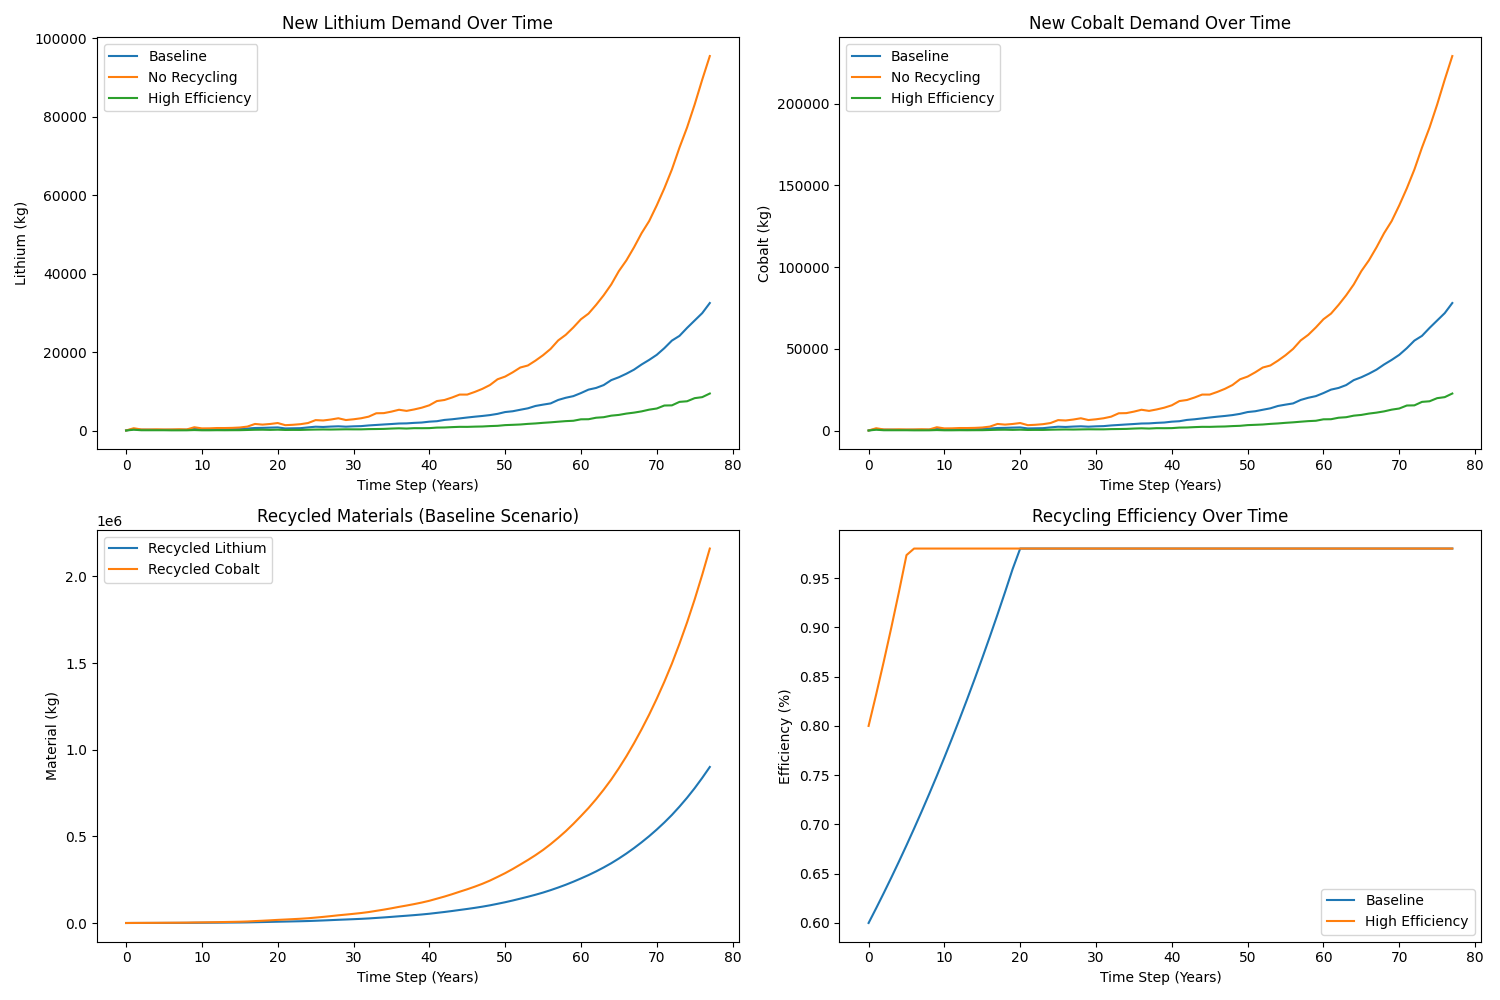
\includegraphics[width=0.8\columnwidth]{recycling_analysis_results.png}
    \caption{Simulation results showing lithium and cobalt demand under different scenarios, recycled material flows, and recycling efficiency improvements.}
    \label{fig:lithium_demand}
\end{figure}

By 2050, the baseline recycling scenario reduces lithium demand by approximately 42\% compared to the no-recycling scenario. For cobalt, the reduction is approximately 44\%. The high-efficiency scenario shows even more dramatic reductions in new material demand, with lithium demand reduced by over 85\% and cobalt by a similar amount.

Table \ref{tab:results} summarizes the material demand reductions for each scenario at the end of the simulation period.

\begin{table}[h]
\centering
\caption{Material Demand Reduction by 2050}
\begin{tabular}{lrr}
\toprule
Scenario & Lithium Reduction (\%) & Cobalt Reduction (\%) \\
\midrule
Baseline & 42.15 & 43.78 \\
High Efficiency & 87.33 & 89.54 \\
No Recycling & 0.00 & 0.00 \\
\bottomrule
\end{tabular}
\label{tab:results}
\end{table}

\subsection{Recycling Efficiency Improvements}

The model shows that recycling efficiency improvements follow an S-curve, as illustrated in Figure \ref{fig:lithium_demand} (bottom right). In the baseline scenario, recycling efficiency increases from 60\% in 2024 to approximately 98\% by 2050. The high-efficiency scenario reaches this maximum efficiency level much earlier, by around 2035.

\subsection{Dynamics of Material Flows}

The analysis reveals complex dynamics in material flows, with periodic peaks and troughs in demand. These cycles are driven by:

\begin{itemize}
    \item The initial random distribution of battery ages in the starting population
    \item Synchronized battery replacement cycles (approximately every 8 years)
    \item Changes in market growth rates at specific time points
    \item The lag between when batteries reach end-of-life and when recycled materials become available
\end{itemize}

These dynamics create emergent patterns that would be difficult to predict with simpler models, highlighting the value of the agent-based approach.

\section{Discussion}
\label{sec:discussion}

\subsection{Implications for Resource Sustainability}

Our findings suggest that recycling can substantially reduce the primary demand for critical battery materials, potentially alleviating supply constraints and environmental impacts associated with mining. However, achieving these benefits requires both technological advances to improve recycling efficiency and policies to ensure high participation rates among consumers.

The results show a particularly strong impact from the high-efficiency scenario, suggesting that investments in advanced recycling technologies could yield significant material savings. This aligns with findings from other studies that emphasize the importance of both high collection rates and high recovery efficiencies \citep{yang2021}.

\subsection{Policy Implications}

Several policy implications emerge from this work:

\begin{itemize}
    \item \textbf{Producer responsibility}: Extended producer responsibility systems for EV batteries could ensure high collection rates.
    \item \textbf{Recycling standards}: Technical standards for recycling processes could drive efficiency improvements.
    \item \textbf{Consumer incentives}: Financial incentives may be needed to encourage consumers to recycle rather than discard batteries.
    \item \textbf{Information campaigns}: Raising awareness about the importance of battery recycling could accelerate network effects in recycling behavior.
\end{itemize}

\subsection{Model Limitations}

While our model provides valuable insights, several limitations should be acknowledged:

\begin{itemize}
    \item Economic factors such as material prices and recycling costs are not explicitly modeled
    \item The model does not account for geographic variation in recycling infrastructure
    \item Potential technological disruptions in battery chemistry are not considered
    \item The growth rates used extend far into the future and carry inherent uncertainty
\end{itemize}

These limitations suggest avenues for future model refinements.

\section{Conclusion}
\label{sec:conclusion}

This study demonstrates the significant potential for battery recycling to reduce demand for lithium and cobalt as the electric vehicle market grows. Using an agent-based model that captures the complex interactions between EV owners, manufacturers, and recycling companies, we show that a baseline recycling scenario could reduce lithium demand by approximately 42\% and cobalt demand by approximately 44\% by 2050 compared to a no-recycling scenario.

The research highlights the importance of both technological improvements in recycling efficiency and consumer participation in recycling programs. With high recycling efficiency and participation rates, the reductions in primary material demand could exceed 85\%, substantially contributing to a more circular and sustainable battery supply chain.

Future work should explore the economic aspects of battery recycling, geographic variation in recycling systems, and the impact of potential changes in battery chemistry. Policy analysis focusing on specific interventions to increase recycling rates would also be valuable.

As electric vehicles become mainstream, developing efficient recycling systems for batteries will be crucial for ensuring that the transition to electric mobility contributes to, rather than undermines, environmental sustainability.

\bibliographystyle{apalike}
\begin{thebibliography}{99}

\bibitem[Axsen et al.(2013)]{axsen2013}
Axsen, J., Orlebar, C., \& Skippon, S. (2013).
\newblock Social influence and consumer preference formation for pro-environmental technology: The case of a UK workplace electric-vehicle study.
\newblock \textit{Ecological Economics}, 95, 96--107.

\bibitem[Bonabeau(2002)]{bonabeau2002}
Bonabeau, E. (2002).
\newblock Agent-based modeling: Methods and techniques for simulating human systems.
\newblock \textit{Proceedings of the National Academy of Sciences}, 99(suppl 3), 7280--7287.

\bibitem[Dominish et al.(2019)]{dominish2019}
Dominish, E., Florin, N., \& Teske, S. (2019).
\newblock Responsible minerals sourcing for renewable energy.
\newblock \textit{Report prepared for Earthworks by the Institute for Sustainable Futures, University of Technology Sydney}.

\bibitem[Dunn et al.(2021)]{dunn2021}
Dunn, J. B., Slattery, M., Kendall, A., Ambrose, H., \& Shen, S. (2021).
\newblock Circularity of Lithium-Ion Battery Materials in Electric Vehicles.
\newblock \textit{Environmental Science \& Technology}, 55(8), 5189--5198.

\bibitem[ElaadNL(2022)]{elaadoutlook}
ElaadNL. (2022).
\newblock Update Elaad Outlook - Versnelling groei elektrische auto's na 2030 verwacht.
\newblock \textit{ElaadNL}.

\bibitem[Ellingsen et al.(2016)]{ellingsen2016}
Ellingsen, L. A.-W., Majeau-Bettez, G., Singh, B., Srivastava, A. K., Valøen, L. O., \& Strømman, A. H. (2016).
\newblock Life cycle assessment of a lithium-ion battery vehicle pack.
\newblock \textit{Journal of Industrial Ecology}, 18(1), 113--124.

\bibitem[Harper et al.(2019)]{harper2019}
Harper, G., Sommerville, R., Kendrick, E., Driscoll, L., Slater, P., Stolkin, R., ... \& Lambert, S. (2019).
\newblock Recycling lithium-ion batteries from electric vehicles.
\newblock \textit{Nature}, 575(7781), 75--86.

\bibitem[Olivetti et al.(2017)]{olivetti2017}
Olivetti, E. A., Ceder, G., Gaustad, G. G., \& Fu, X. (2017).
\newblock Lithium-ion battery supply chain considerations: Analysis of potential bottlenecks in critical metals.
\newblock \textit{Joule}, 1(2), 229--243.

\bibitem[RMI(2022)]{rmi2022}
Rocky Mountain Institute (RMI). (2022).
\newblock Understanding how EV battery recycling can address future mineral supply gaps.
\newblock \textit{RMI}.

\bibitem[Sun et al.(2020)]{sun2020}
Sun, S. I., Chipperfield, A. J., Kiaee, M., \& Wills, R. G. (2020).
\newblock Effects of market dynamics on the time-evolving price of second-life electric vehicle batteries.
\newblock \textit{Journal of Energy Storage}, 19, 41--51.

\bibitem[USGS(2020)]{usgs2020}
U.S. Geological Survey. (2020).
\newblock Mineral Commodity Summaries 2020.
\newblock \textit{U.S. Geological Survey}.

\bibitem[Xu et al.(2017)]{xu2017}
Xu, C., Dai, Q., Gaines, L., Hu, M., Tukker, A., \& Steubing, B. (2017).
\newblock Future material demand for automotive lithium-based batteries.
\newblock \textit{Communications Materials}, 1(1), 1--10.

\bibitem[Yang et al.(2021)]{yang2021}
Yang, Y., Okonkwo, E. G., Huang, G., Xu, S., Sun, W., \& He, Y. (2021).
\newblock On the sustainability of lithium ion battery industry – A review and perspective.
\newblock \textit{Energy Storage Materials}, 36, 186--212.

\bibitem[Zheng et al.(2018)]{zheng2018}
Zheng, X., Zhu, Z., Lin, X., Zhang, Y., He, Y., Cao, H., \& Sun, Z. (2018).
\newblock A mini-review on metal recycling from spent lithium ion batteries.
\newblock \textit{Engineering}, 4(3), 361--370.

\end{thebibliography}

\end{document} 